\documentclass{article}
\usepackage[utf8]{inputenc}
\usepackage{subfig}

%References
\usepackage{natbib}
%IMPORTANT use https://www.citationmachine.net/ if you need to generate references!
% \citep{reference} creates Harvard Style references throughout

%Colors
\usepackage{xcolor}

\usepackage[protrusion=true,expansion]{microtype}

%Code Markup
\usepackage[outputdir=cache]{minted}
%Syntax Highlighting Style
\definecolor{bggray}{RGB}{40,40,40}
\newmintedfile[javacode]{java}{
	style=fruity,
	bgcolor=bggray,
	linenos,
	breaklines,
	tabsize=2,
	obeytabs
}

\newmintedfile[bashoutput]{text} {
	style=fruity,
	bgcolor=bggray,
	breaklines,
	tabsize =2,
	obeytabs
}

\newmintedfile[armfile]{ARM} {
	style=fruity,
	bgcolor=bggray,
	breaklines,
	tabsize =2,
	obeytabs
}

%Page Margins and stuff
\usepackage{geometry}
 \geometry{
 a4paper,
 total={170mm,257mm},
 left=20mm,
 }

%Pictures
\usepackage{graphicx}
\graphicspath{ {./images/} }

%Move the title position
\usepackage{titling}

\setlength{\droptitle}{-8.5em} %Up, near the top but not too high

\title{Assignment 5 - CT2109 Object Oriented Programming: Data Structures and Algorithms}
\author{Daniel Hannon (19484286)}
\date{May 2021}

\begin{document}
	\maketitle
	%Sets to Harvard Style and links the references file
	\section{Problem Analysis}
	\subsection{Overview}
	Brief:\textit{"For this assignment, you will use the BinaryTree implementation on Blackboard to program a guessing game. Firstly, you will manually build an initial tree in which each internal node is a yes/no question. Yes goes to left side(left child), No goes to right side(right child).Each leaf nodein the tree is a guess. If the user arrives at a leaf node and the guess is wrong, get the user to provide you with what the correct answer actually was and to provide a new yes/no question which can be added to the tree."}
	\subsection{Part 1: Getting the questions to work}
	The main part of this was implementing \textit{\textbf{BinaryNodeInterface}<\textbf{T}>} which was quite simple. the only Alteration I made to it was I overrode the \textit{toString()} method for my implementation but this will be explained later. \textit{getHeight()}, \textit{getNumberOfNodes()}, and \textit{copy()} were all implemented using Recursion for speed.\\
	Once I had the Binary Tree implemented, It was a matter of constructing a test tree. Logically the tree needed to be built from the results backwards so that wasn't the hardest thing to do, once that was done it was a matter of getting user input.\\
	in order to make the input more flexible I forced it to be lowercase once input had been scanned and then it was compared to longform and shortform of yes/no.
	\subsection{Part 2: Adding in new questions}
	In order to avoid the need to perform a binary search at the end if you had to input a new question/answer, the question and answer are sanitized, I saved the position of the previous node and the direction you took when you responded. Then a new branch is created, the leaf which was formerly in that position in the tree is added to the new branch and that branch is inserted where that leaf used to be.
	\newpage
	\subsection{Part 3: Saving}
	\begin{figure}[h!]
	\centering
	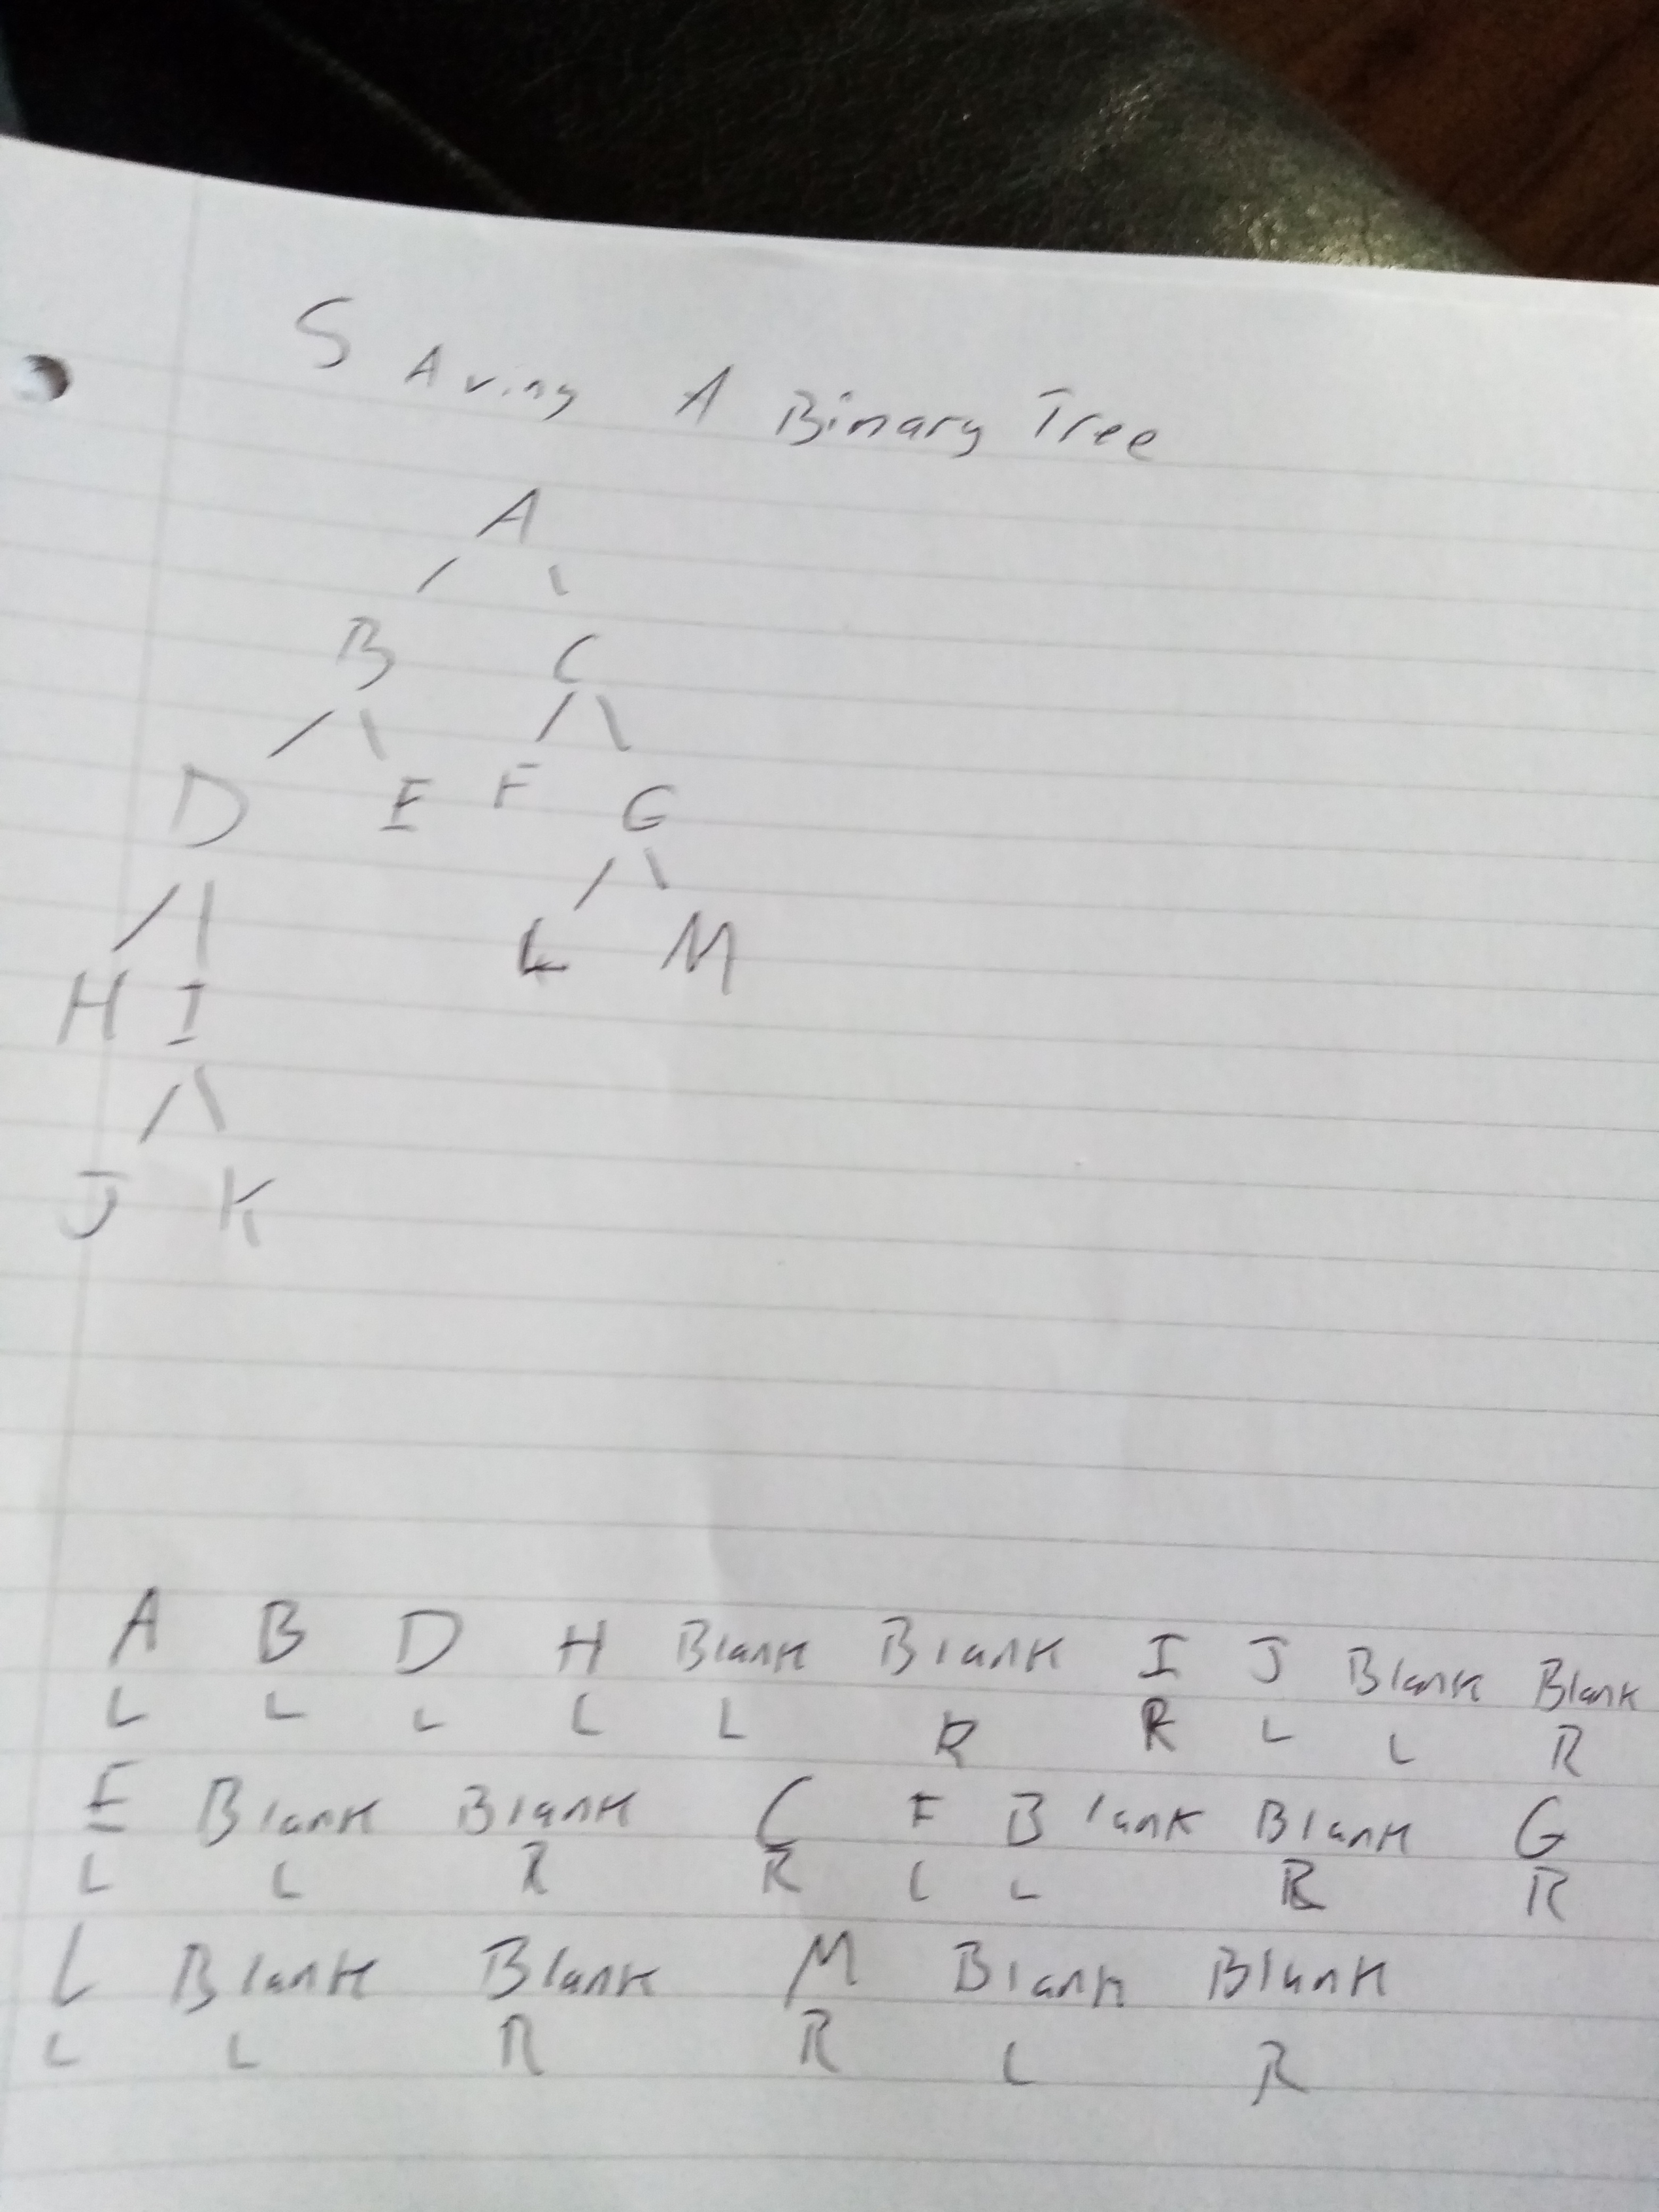
\includegraphics[width=0.4\textwidth]{btree.jpg}
	\caption{Binary Tree and potential save schema}
	\end{figure}
	Saving was a matter of Finding a way to serialize the Binary Tree and then dumping this in a textfile. I figured the easiest way to serialize it would be to overwrite the \textit{toString()} method and have it return the nodes in comma separated form, where left hand nodes are printed first until a null is found which is represented as "\#" and then it prints the right hand nodes, this runs recursively of course. I then utilize a \textbf{FileWriter} and place it all in \textit{saveFile.txt}
	\subsection{Part 4: Loading}
	Loading the file and keeping the structure was initally somewhat challenging as I had planned to use 3 Stacks and done some weird stuff but ultimately I achieved it by using a single Stack.\\
	In order to load it I felt the easiest way would be to split savestring at every comma and work backwards, if two elements in a row were "\#" it creates a leafnode using the element after the "\#" in the search, this is then added to the stack. where if it lands on an element that is not "\#" it pulls two elements from the Stack, creates a new branch using the current element as the data and the two recently pulled from the stack as it's branches/leaves. Once the entire array had been iterated through, the top element in the stack is returned.\\
	As all elements either have two children or none I was able to reduce the amount of required checks for it to run to success.
	\newpage
	\section{Code}
	Binary Tree implementation
	\javacode{TreeNode.java}
	Main file
	\javacode{Main.java}
	\section{Testing}
	\begin{figure}[h!]
	\centering
	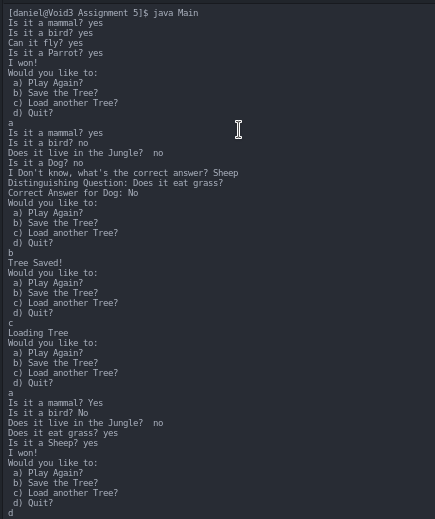
\includegraphics{test1}
	\end{figure}
	\bibliographystyle{agsm}
	\bibliography{references}
\end{document}
